%bra paket
\documentclass[twocolumn]{article}
\usepackage[utf8]{inputenc}
%\usepackage[swedish]{babel}
\usepackage{fancyhdr}
%\usepackage{times}
%\usepackage{alltt} %verbatim text med möjlighet till andra latexkommandon i.
%\usepackage[usenames,dvipsnames]{color} %fler färger att välja på
%\usepackage{wrapfig} %figurer som ligger sida vid sida med texten
%\usepackage[table]{xcolor} %bakgrundsfärg i tabeller
%\usepackage[small,compact]{titlesec} %Spara plats!!
\usepackage{amsmath}
\usepackage{multicol}
\usepackage{graphicx}
\usepackage{float} %gör så att man kan placera bilder exakt mha [H]
\usepackage[table]{xcolor} %bakgrundsfärg i tabeller

%\usepackage[ddmmyyyy]{datetime}

\usepackage{setspace}
%\usepackage[usenames,dvipsnames]{color} %fler färger att välja på
%\usepackage{pdfpages} %för att kunna använda includepdf i appendix
\usepackage{pgf}
\usepackage{tikz}
\usetikzlibrary{arrows,automata}
\usetikzlibrary{positioning}
\tikzset{
    state/.style={
           rectangle,
           draw=black, thick,
           minimum height=3em,
           inner sep=5pt,
           text centered,
           },
}

% Different font in captions
\newcommand{\captionfonts}{\em}
\makeatletter  % Allow the use of @ in command names
\long\def\@makecaption#1#2{%
  \vskip\abovecaptionskip
  \sbox\@tempboxa{{\captionfonts #1: #2}}%
  \ifdim \wd\@tempboxa >\hsize
    {\captionfonts #1: #2\par}
  \else
    \hbox to\hsize{\hfil\box\@tempboxa\hfil}%
  \fi
  \vskip\belowcaptionskip}
\makeatother   % Cancel the effect of \makeatletter


%marginaler
\setlength\topmargin{0in}
\setlength\headheight{11pt}
\setlength\textheight{8.1in}
\setlength\textwidth{6.5in}
\setlength\oddsidemargin{0in}
\setlength\evensidemargin{0in}
\setlength\parindent{0in}
\setlength\parskip{0in}
\frenchspacing %Oui!

%För att kunna typsätta delar för sig!
\newcommand{\master}{}

%då kör vi


\begin{document}
%%%%%%%%%%%%%%%%%%% Försättsblad %%%%%%%%%%%%%%%%%%%%%%%%
\begin{titlepage}
\title{\textbf{Electric lab-assistant} \\
\Large{Engineering Applications using Matlab}\\
\large{TNG016}}
\author{
\vspace{30pt}\\
\large
ED3:\bigskip \\
\begin{tabular}{l l}
	Dan	Helgesson & danhe046 \\
	Albert Skog	& albsk635 \\
	Karl Westerberg	& karwe772 \\
\end{tabular}\vspace{40pt}\\
Examiner: Qingxiang Zhao 
}
\date{Submitted: \today}
\maketitle
\thispagestyle{empty}
\begin{center}


\begin{figure}[b]
	\begin{center}
		
\includegraphics[scale=0.6]{Figure/LIU-logo.jpg}
	\end{center}
\end{figure}

\end{center}

\end{titlepage}

%%%%%%%%%%%%%%%%%%% Header %%%%%%%%%%%%%%%%%%%%%%%
\pagestyle{fancy}
\fancyhead[l]{Engineering Applications using Matlab\\Electric Lab-Assistant}
\fancyhead[r]{Dan Helgesson, Albert Skog\\ \& Karl Westerberg}

%%%%%%%%%%%%%%%%%% Rapporten %%%%%%%%%%%%%%%%%%%%%
\section{Introduction}
%Om filen typsätts som del av hela rapporten så finns \master definierat i början och ingen \begin{document} och \end{document} får finnas, men för att kunna typsätta filen för sig är dem ett måste! \newcommand{\master}{} krävs i början på huvudrapporten!
\ifdefined\master
\else
	\documentclass[twocolumn]{article}
	\input{../preamble}
	\begin{document}
\fi
%text goes here!









\ifdefined\master
\else
	\end{document}
\fi

\section{Lab-Assistant}

The user interface of Lab-Assistant is designed to be intuitive and user-friendly. When launched the user is met by three empty columns, each with a popup-menu at the top. The columns are called \emph{input}, \emph{output} and \emph{export}, each with a set of 3-4 different options. Using different combinations of these options, a variety of tasks can be performed.
%Om filen typsätts som del av hela rapporten så finns \master definierat i början och ingen \begin{document} och \end{document} får finnas, men för att kunna typsätta filen för sig är dem ett måste! \newcommand{\master}{} krävs i början på huvudrapporten!
\ifdefined\master
\else
	\documentclass[twocolumn]{article}
	%\input{../preamble}
	\begin{document}
\fi
\subsection{Inputs}
Lab Assistant supports two types of devices for input; function generators and voltage generators. The function generator can also be used to generate a frequency sweep.
\subsubsection*{Function Generator}
Uses function generator to output a signal. The \emph{waveform} popup-menu sets the signal type to sine, square, triangle or sawtooth. If no waveform is selected the current waveform of the function generator is used. \emph{Frequency}, \emph{amplitude} and \emph{offset} controlls the parameters of the output. In order to establish a connection to the function generator its GPIB-address must be put into the \emph{GPIB-address} field.

\subsubsection*{Frequency Sweep}
The function generator can also be used to generate a Bode plot of a connected system. When \emph{frequency sweep} is selected as input, output is automatically set to \emph{bode graph} and no other outputs can be chosen. Available settings for the sweep are \emph{start frequency}, \emph{end frequency}, \emph{step length} and \emph{amplitude}. GPIB-address must allso be filled in as described above.

\subsubsection*{Voltage Generator}
The other device supported is the voltage generator. Apart from \emph{GPIB-Address} of the voltage generator, the available settings are \emph{voltage} and \emph{current limit}. Output can be toggled with the \emph{output on/off} pushbutton.


\ifdefined\master
\else
	\end{document}
\fi
%Om filen typsätts som del av hela rapporten så finns \master definierat i början och ingen \begin{document} och \end{document} får finnas, men för att kunna typsätta filen för sig är dem ett måste! \newcommand{\master}{} krävs i början på huvudrapporten!
\ifdefined\master
\else
	\documentclass[twocolumn]{article}
	\usepackage{graphicx}
	\usepackage{float}
	\usepackage{alltt}
	\begin{document}
\fi

\subsection{Outputs}
Two methods of gathering output data are available

\subsubsection*{Oscilloscope}
The oscilloscope has two functions, \emph{picture} and \emph{measurement} shown in Figure \ref{fig:osc}. The picture option practicaly takes a copy of the oscilloscope screen and shows it in the panel. The measurement option is used for getting the graph and plot with Matlab without all extra information the oscilloscope shows. The plot is then displayed in the panel. After entering the \emph{GPIB address} for the oscilloscope, the \emph{Start} button will execute the option chosen. (Figure \ref{fig:osc})

\begin{figure}[H]
\centering
\fbox{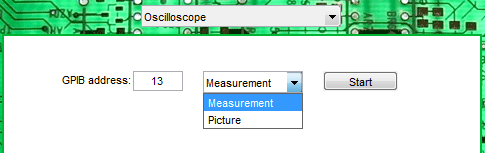
\includegraphics[width=6cm]{Figure/out_oscilloscope.png}}
\caption{Oscilloscope output settings.}
\label{fig:osc}
\end{figure}

\subsubsection*{Multimeter}
The multimeter function is just a multimeter, that displays the value in the panel as shown in Figure \ref{fig:multi}. When the \emph{Start} button is hit the multimeter begins uppdating the value in the panel. When the \emph{Stop} button is hit the multimeter stops updating and instead plot all previous values in a stem plot. (Figure \ref{fig:multi})

\begin{figure}[H]
\centering
\fbox{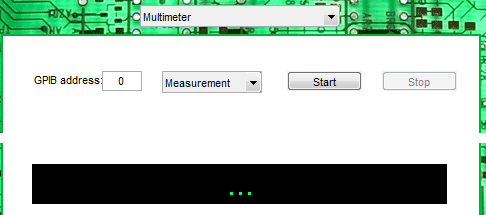
\includegraphics[width=7cm]{Figure/Multimeter.png}}
\caption{Multimeter output settings.}
\label{fig:multi}
\end{figure}

\subsubsection*{Bode Graph}
When the frequency sweep is chosen in the input panel it automaticaly chose the bode graph in the output panel. The Bode Graph only works with the frequency sweep as the start button is placed in the input panel. The plot is shown in the output panel. (Figure \ref{fig:bode})

\begin{figure}[H]
\centering
\fbox{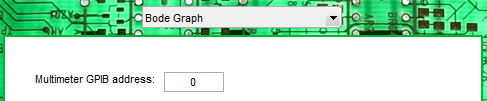
\includegraphics[width=6cm]{Figure/bode_graph.png}}
\caption{Bode plot output settings.}
\label{fig:bode}
\end{figure}


\ifdefined\master
\else
	\end{document}
\fi
%Om filen typsätts som del av hela rapporten så finns \master definierat i början och ingen \begin{document} och \end{document} får finnas, men för att kunna typsätta filen för sig är dem ett måste! \newcommand{\master}{} krävs i början på huvudrapporten!
\ifdefined\master
\else
	\documentclass[twocolumn]{article}
	%\input{preamble}
	\begin{document}
\fi
\subsection{Exports}
The program has four different choices for exporting the obtained data; copy to clipboard, save as image, create LaTeX report and create Microsoft Word report.

\subsection*{Clipboard}
Copies the figure to clipboard. Textboxes enable the user to modify title and axis labels before copying.

\subsection*{Image}
Saves the image to disk. Textboxes enable the user to modify title and axis labels before copying.

\subsection*{LaTeX}
Generates LaTeX report containing the figure. \emph{Image name} textbox enables user to choose file name and format for the figure, which will be saved at the same location as the tex-file. \emph{Caption}, \emph{label} and \emph{width} properties are transferred to corresponding LaTeX commands, while tite and labels are applied directly to the figure before exporting. 

\subsection*{Word}
Generates Microsoft Word report containing the figure. \emph{Title}, \emph{x-label} and \emph{y-label} overrides the settings of the figure and the caption is inserted on a centred line below.




\ifdefined\master
\else
	\end{document}
\fi

\section{Examples}

\section{Conclusion}

\end{document}